\documentclass[mathserif,8pt]{beamer}
\usepackage{indentfirst,mathrsfs}
\usepackage{amssymb}
\usepackage{pifont}
\usepackage{amsfonts}
\usepackage{booktabs}
\usepackage{color} 
\usepackage{bbm}
\usepackage{graphicx} 
\usepackage{indentfirst,mathrsfs}
\setbeamertemplate{footline}[frame number]

\usetheme{Darmstadt}

\usepackage{times}
\usefonttheme{structurebold}

\usepackage[english]{babel}
\usepackage{pgf,pgfarrows,pgfnodes,pgfautomata,pgfheaps}
\usepackage{amsmath,amssymb,mathrsfs}
\usepackage[latin1]{inputenc}
\usepackage{color}
\beamertemplatetextbibitems
\setbeamercovered{dynamic}



\definecolor{rgb0}{rgb}{1.0,0.5,0.5}
\definecolor{rgb1}{rgb}{0.0,0.5,0.5}
\definecolor{rgb2}{rgb}{0.8,0.6,0.6}
\definecolor{rgb3}{rgb}{0.1,0.7,0.6}

\newtheorem{property}{Property}

\newtheorem{construction}{Construction}
\newtheorem{proposition}{Proposition}




\pgfdeclaremask{tu}{beamer-tu-logo-mask}
\pgfdeclaremask{computer}{beamer-computer-mask}
\pgfdeclareimage[interpolate=true,mask=computer,height=2cm]{computerimage}{beamer-computer}
\pgfdeclareimage[interpolate=true,mask=computer,height=2cm]{computerworkingimage}{beamer-computerred}
\pgfdeclareimage[mask=tu,height=.5cm]{logo}{beamer-tu-logo}

\logo{\pgfuseimage{logo}}
\title{Automatic Security Evaluation of Block Cipher}

\author{Liu Zhang}
\institute{School of Cyber Engineering, Xidian University}
\colorlet{redshaded}{red!25!bg} \colorlet{shaded}{black!25!bg}
\colorlet{shadedshaded}{black!10!bg}
\colorlet{blackshaded}{black!40!bg}

\colorlet{darkred}{red!80!black} \colorlet{darkblue}{blue!80!black}
\colorlet{darkgreen}{green!80!black}

\def\radius{0.96cm}
\def\innerradius{0.85cm}

\def\softness{0.4}
\definecolor{softred}{rgb}{1,\softness,\softness}
\definecolor{softgreen}{rgb}{\softness,1,\softness}
\definecolor{softblue}{rgb}{\softness,\softness,1}

\definecolor{softrg}{rgb}{1,1,\softness}
\definecolor{softrb}{rgb}{1,\softness,1}
\definecolor{softgb}{rgb}{\softness,1,1}

\newcommand{\Bandshaded}[2]{
  \color{shadedshaded}
  \pgfmoveto{\pgfxy(-0.5,0)}
  \pgflineto{\pgfxy(-0.6,0.1)}
  \pgflineto{\pgfxy(-0.4,0.2)}
  \pgflineto{\pgfxy(-0.6,0.3)}
  \pgflineto{\pgfxy(-0.4,0.4)}
  \pgflineto{\pgfxy(-0.5,0.5)}
  \pgflineto{\pgfxy(4,0.5)}
  \pgflineto{\pgfxy(4.1,0.4)}
  \pgflineto{\pgfxy(3.9,0.3)}
  \pgflineto{\pgfxy(4.1,0.2)}
  \pgflineto{\pgfxy(3.9,0.1)}
  \pgflineto{\pgfxy(4,0)}
  \pgfclosepath
  \pgffill

  \color{black}
  \pgfputat{\pgfxy(0,0.7)}{\pgfbox[left,base]{#1}}
  \pgfputat{\pgfxy(0,-0.1)}{\pgfbox[left,top]{#2}}
}

\newcommand{\Band}[2]{
  \color{shaded}
  \pgfmoveto{\pgfxy(-0.5,0)}
  \pgflineto{\pgfxy(-0.6,0.1)}
  \pgflineto{\pgfxy(-0.4,0.2)}
  \pgflineto{\pgfxy(-0.6,0.3)}
  \pgflineto{\pgfxy(-0.4,0.4)}
  \pgflineto{\pgfxy(-0.5,0.5)}
  \pgflineto{\pgfxy(4,0.5)}
  \pgflineto{\pgfxy(4.1,0.4)}
  \pgflineto{\pgfxy(3.9,0.3)}
  \pgflineto{\pgfxy(4.1,0.2)}
  \pgflineto{\pgfxy(3.9,0.1)}
  \pgflineto{\pgfxy(4,0)}
  \pgfclosepath
  \pgffill

  \color{black}
  \pgfputat{\pgfxy(0,0.7)}{\pgfbox[left,base]{#1}}
  \pgfputat{\pgfxy(0,-0.1)}{\pgfbox[left,top]{#2}}
}

\newcommand{\BaenderNormal}
{%
  \pgfsetlinewidth{0.4pt}
  \color{black}
  \pgfputat{\pgfxy(0,5)}{\Band{input tapes}{}}
  \pgfputat{\pgfxy(0.35,4.6)}{\pgfbox[center,base]{$\vdots$}}
  \pgfputat{\pgfxy(0,4)}{\Band{}{}}

  \pgfxyline(0,5)(0,5.5)
  \pgfxyline(1.2,5)(1.2,5.5)
  \pgfputat{\pgfxy(0.25,5.25)}{\pgfbox[left,center]{$w_1$}}

  \pgfxyline(0,4)(0,4.5)
  \pgfxyline(1.8,4)(1.8,4.5)
  \pgfputat{\pgfxy(0.25,4.25)}{\pgfbox[left,center]{$w_n$}}
  \ignorespaces}

\newcommand{\BaenderZweiNormal}
{%
  \pgfsetlinewidth{0.4pt}
  \color{black}
  \pgfputat{\pgfxy(0,5)}{\Band{Zwei Eingabebader}{}}
  \pgfputat{\pgfxy(0,4.25)}{\Band{}{}}

  \pgfxyline(0,5)(0,5.5)
  \pgfxyline(1.2,5)(1.2,5.5)
  \pgfputat{\pgfxy(0.25,5.25)}{\pgfbox[left,center]{$u$}}

  \pgfxyline(0,4.25)(0,4.75)
  \pgfxyline(1.8,4.25)(1.8,4.75)
  \pgfputat{\pgfxy(0.25,4.5)}{\pgfbox[left,center]{$v$}}
  \ignorespaces}

\newcommand{\BaenderHell}
{%
  \pgfsetlinewidth{0.4pt}
  \color{black}
  \pgfputat{\pgfxy(0,5)}{\Bandshaded{input tapes}{}}
  \color{shaded}
  \pgfputat{\pgfxy(0.35,4.6)}{\pgfbox[center,base]{$\vdots$}}
  \pgfputat{\pgfxy(0,4)}{\Bandshaded{}{}}

  \color{blackshaded}
  \pgfxyline(0,5)(0,5.5)
  \pgfxyline(1.2,5)(1.2,5.5)
  \pgfputat{\pgfxy(0.25,5.25)}{\pgfbox[left,center]{$w_1$}}

  \pgfxyline(0,4)(0,4.5)
  \pgfxyline(1.8,4)(1.8,4.5)
  \pgfputat{\pgfxy(0.25,4.25)}{\pgfbox[left,center]{$w_n$}}
  \ignorespaces}

\newcommand{\BaenderZweiHell}
{%
  \pgfsetlinewidth{0.4pt}
  \color{black}
  \pgfputat{\pgfxy(0,5)}{\Bandshaded{Zwei Eingabebader}{}}%
  \color{blackshaded}
  \pgfputat{\pgfxy(0,4.25)}{\Bandshaded{}{}}
  \pgfputat{\pgfxy(0.25,4.5)}{\pgfbox[left,center]{$v$}}
  \pgfputat{\pgfxy(0.25,5.25)}{\pgfbox[left,center]{$u$}}%

  \pgfxyline(0,5)(0,5.5)
  \pgfxyline(1.2,5)(1.2,5.5)

  \pgfxyline(0,4.25)(0,4.75)
  \pgfxyline(1.8,4.25)(1.8,4.75)
  \ignorespaces}

\newcommand{\Slot}[1]{%
  \begin{pgftranslate}{\pgfpoint{#1}{0pt}}%
    \pgfsetlinewidth{0.6pt}%
    \color{structure}%
    \pgfmoveto{\pgfxy(-0.1,5.5)}%
    \pgfbezier{\pgfxy(-0.1,5.55)}{\pgfxy(-0.05,5.6)}{\pgfxy(0,5.6)}%
    \pgfbezier{\pgfxy(0.05,5.6)}{\pgfxy(0.1,5.55)}{\pgfxy(0.1,5.5)}%
    \pgflineto{\pgfxy(0.1,4.0)}%
    \pgfbezier{\pgfxy(0.1,3.95)}{\pgfxy(0.05,3.9)}{\pgfxy(0,3.9)}%
    \pgfbezier{\pgfxy(-0.05,3.9)}{\pgfxy(-0.1,3.95)}{\pgfxy(-0.1,4.0)}%
    \pgfclosepath%
    \pgfstroke%
  \end{pgftranslate}\ignorespaces}

\newcommand{\SlotZwei}[1]{%
  \begin{pgftranslate}{\pgfpoint{#1}{0pt}}%
    \pgfsetlinewidth{0.6pt}%
    \color{structure}%
    \pgfmoveto{\pgfxy(-0.1,5.5)}%
    \pgfbezier{\pgfxy(-0.1,5.55)}{\pgfxy(-0.05,5.6)}{\pgfxy(0,5.6)}%
    \pgfbezier{\pgfxy(0.05,5.6)}{\pgfxy(0.1,5.55)}{\pgfxy(0.1,5.5)}%
    \pgflineto{\pgfxy(0.1,4.25)}%
    \pgfbezier{\pgfxy(0.1,4.25)}{\pgfxy(0.05,4.15)}{\pgfxy(0,4.15)}%
    \pgfbezier{\pgfxy(-0.05,4.15)}{\pgfxy(-0.1,4.2)}{\pgfxy(-0.1,4.25)}%
    \pgfclosepath%
    \pgfstroke%
  \end{pgftranslate}\ignorespaces}

\newcommand{\ClipSlot}[1]{%
  \pgfrect[clip]{\pgfrelative{\pgfxy(-0.1,0)}{\pgfpoint{#1}{4cm}}}{\pgfxy(0..2,1.5)}\ignorespaces}

\newcommand{\ClipSlotZwei}[1]{%
  \pgfrect[clip]{\pgfrelative{\pgfxy(-0.1,0)}{\pgfpoint{#1}{4.25cm}}}{\pgfxy(0.2,1.25)}\ignorespaces}


\AtBeginSection[]{\frame{\frametitle{Outline}\tableofcontents[current]}}
\begin{document}

\frame{\titlepage}

%\part{Main Part}
%\frame{\frametitle{Outline}\tableofcontents[part=1]}

\section{Block Cipher}
\frame { \frametitle{Block Cipher}
	\begin{figure}[h]
	\centering  
	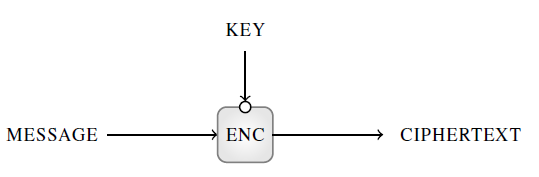
\includegraphics[width=0.6\linewidth]{block-cipher.PNG}  
		\caption{The process of encryption}  
	\end{figure}
	A block cipher has two important parameters:
	\begin{itemize}
		\item the $ block size $, which will be denoted by $ \mathbf{b}  $, and
		\item the $ key size $, which will be denoted by $ \mathbf{k} $.
	\end{itemize}
}

\frame { \frametitle{Structure of Block Cipher}

	\begin{figure} 
		\begin{minipage}[t]{0.5\linewidth} 
			\centering 
			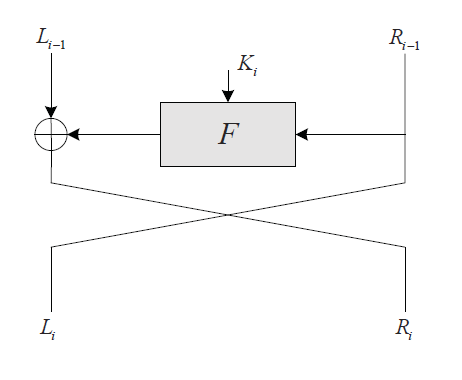
\includegraphics[width=2.0in]{Feistel-Structure.PNG} 
			\caption{Feistel-Structure} 
			\label{frame} 
		\end{minipage}% 
		\begin{minipage}[t]{0.5\linewidth} 
			\centering 
			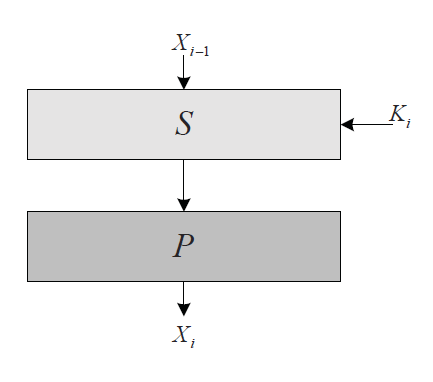
\includegraphics[width=1.8in]{SP-Structure.PNG} 
			\caption{SP-Structure} 
			\label{label} 
		\end{minipage} 
	\end{figure}

}
\frame { \frametitle{Present}
	\begin{figure}[h]
		\centering  
		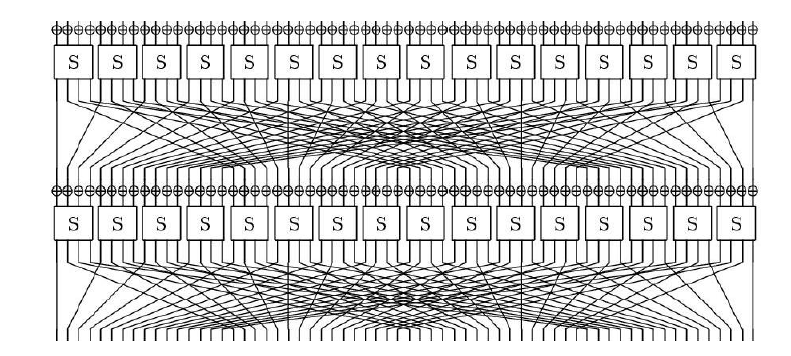
\includegraphics[width=0.8\linewidth]{Present-80.PNG}  
		\caption{Two consecutive rounds of Present-80 encryption process}  
	\end{figure}
}
\frame { \frametitle{Differential Model of Sbox}
	\begin{figure}[h]
		\centering  
		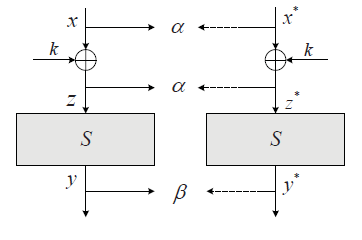
\includegraphics[width=0.5\linewidth]{differential-model-of-sbox.PNG}  
		\caption{Differential Model of Sbox}  
	\end{figure}

	\begin{figure}[h]
	\centering  
	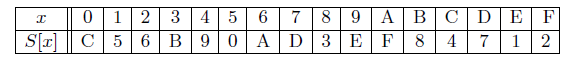
\includegraphics[width=0.6\linewidth]{Present-sbox.PNG}  
	\caption{The S-box of Present}  
\end{figure}
}
\frame { \frametitle{The Differential Distribution Table of Present S-box}
	\begin{figure}[h]
		\centering  
		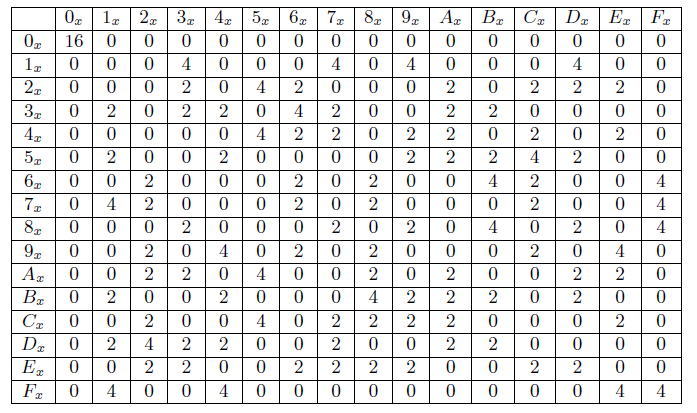
\includegraphics[width=0.8\linewidth]{ddt-present.PNG}  
		\caption{The Differential Distribution Table of Present S-box}  
	\end{figure}
}

\section{Differential Cryptanalysis of a Toy Cipher}
\frame { \frametitle{Differential Cryptanalysis of a Toy Cipher}
\begin{figure} 
	\begin{minipage}[t]{0.5\linewidth} 
		\centering 
		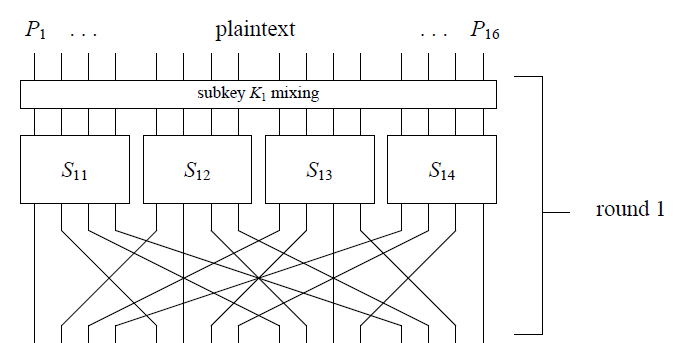
\includegraphics[width=2.1in]{round-1.PNG} 
		\caption{Round-1} 
		\label{frame} 
	\end{minipage}% 
	\begin{minipage}[t]{0.5\linewidth} 
		\centering 
		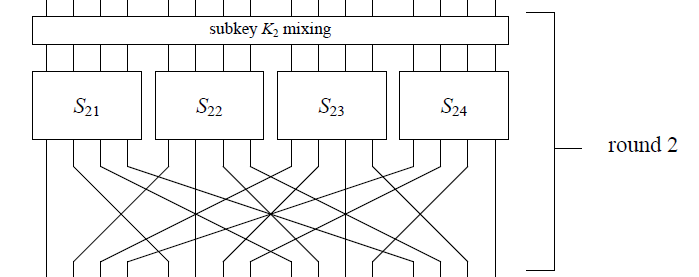
\includegraphics[width=2.1in]{round-2.PNG} 
		\caption{Round-2} 
		\label{label} 
	\end{minipage} 
\end{figure}

\begin{figure} 
	\begin{minipage}[t]{0.5\linewidth} 
		\centering 
		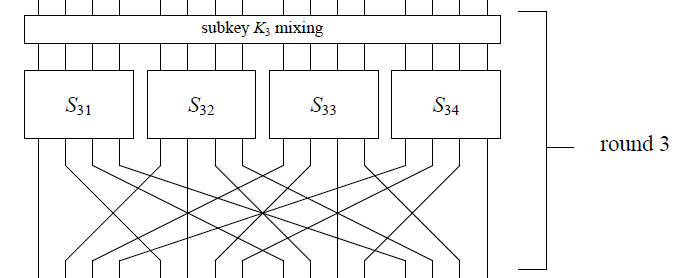
\includegraphics[width=2.1in]{round-3.PNG} 
		\caption{Round-3} 
		\label{frame} 
	\end{minipage}% 
	\begin{minipage}[t]{0.5\linewidth} 
		\centering 
		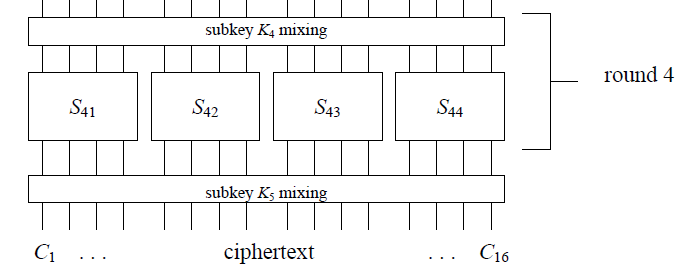
\includegraphics[width=2.1in]{round-4.PNG} 
		\caption{Round-4} 
		\label{label} 
	\end{minipage} 
\end{figure}
}
\frame { \frametitle{Differential Cryptanalysis of a Toy Cipher}
\begin{itemize}
	\item S-box Representation of Toy Cipher
	~ \\
	~ \\
	\begin{figure}[h]
		\centering  
		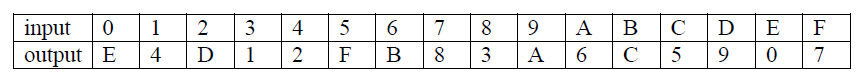
\includegraphics[width=0.8\linewidth]{S-box-of-toy-cipher.PNG}
	\end{figure}
	~ \\
	\item Permutation of Toy Cipher
	~ \\
	~ \\
		\begin{figure}[h]
		\centering  
		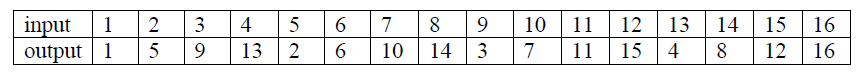
\includegraphics[width=0.8\linewidth]{permutation-of-toy-cipher.PNG}
	\end{figure}
\end{itemize}
}

\frame { \frametitle{Differential Cryptanalysis of a Toy Cipher}
\begin{figure}[h]
	\centering  
	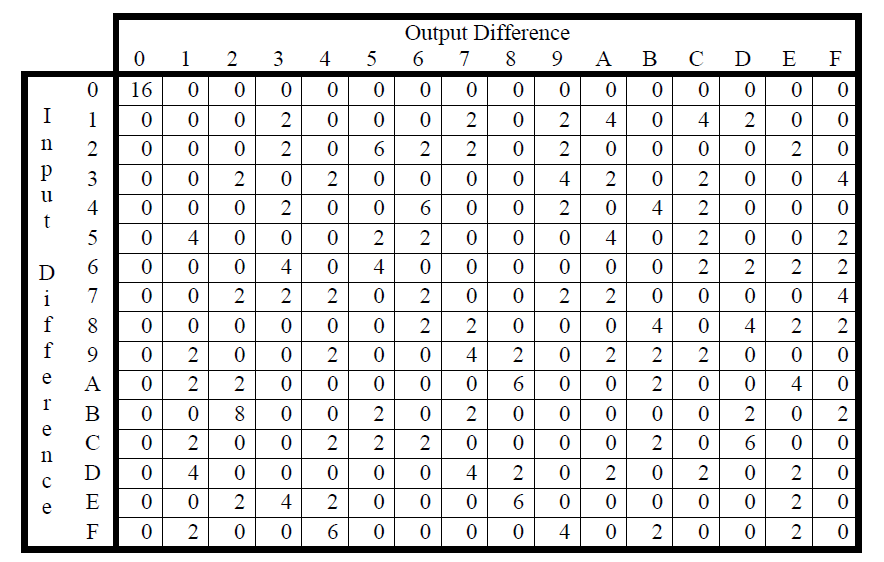
\includegraphics[width=0.8\linewidth]{ddt-toy-cipher.PNG}
	\caption{Difference Distribution Table}
\end{figure}

}

\frame { \frametitle{Differential Cryptanalysis of a Toy Cipher}
	\begin{figure} 
		\begin{minipage}[t]{0.5\linewidth} 
			\centering 
			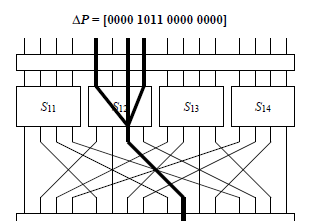
\includegraphics[width=1.8in]{dc1.PNG} 
			\caption{Round-1} 
			\label{frame} 
		\end{minipage}% 
		\begin{minipage}[t]{0.5\linewidth} 
			\centering 
			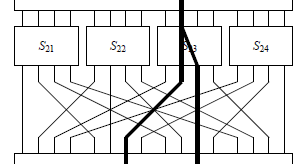
\includegraphics[width=1.8in]{dc2.PNG} 
			\caption{Round-2} 
			\label{label} 
		\end{minipage} 
	\end{figure}
	
	\begin{figure} 
		\begin{minipage}[t]{0.5\linewidth} 
			\centering 
			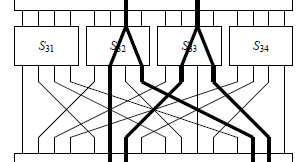
\includegraphics[width=1.8in]{dc3.PNG} 
			\caption{Round-3} 
			\label{frame} 
		\end{minipage}% 
		\begin{minipage}[t]{0.5\linewidth} 
			\centering 
			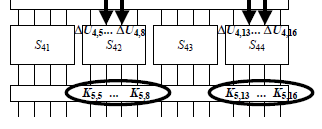
\includegraphics[width=1.8in]{dc4.PNG} 
			\caption{Round-4} 
			\label{label} 
		\end{minipage} 
	\end{figure}
}
\frame { \frametitle{Differential Cryptanalysis of a Toy Cipher}
  	We use the follwing difference pairs of the S-box:
	\begin{itemize}
		\item $S_{12}:\Delta X =B \rightarrow \Delta Y =2 $ with probability  8/16
		~ \\
		\item $S_{12}:\Delta X =4 \rightarrow \Delta Y =6 $ with probability  6/16
		~ \\
		\item $S_{12}:\Delta X =2 \rightarrow \Delta Y =5 $ with probability  6/16
		~ \\
		\item $S_{12}:\Delta X =2 \rightarrow \Delta Y =5 $ with probability  6/16	
	\end{itemize}

	The input difference and output difference to the every round
	\begin{itemize}
		\item $\Delta P=\Delta U_{1} =[0000 \  1011 \ 0000 \ 0000] $ with probability  8/16
		~ \\
		\item $\quad \quad \quad \Delta V_{1} =[0000 \  0010 \ 0000 \ 0000] $
		~ \\
		\item $\quad \quad \quad \Delta U_{2} =[0000 \  0000 \ 0100 \ 0000] $ with probability  6/16
		~ \\
		\item  $\quad \quad \quad \Delta V_{2} =[0000 \  0000 \ 0110 \ 0000] $
		~ \\
		\item $\quad \quad \quad \Delta U_{3} =[0000 \  0010 \ 0010 \ 0000] $ with probability  (6/16)*(6/16)
		~ \\
		\item  $\quad \quad \quad \Delta V_{3} =[0000 \  0101 \ 0101 \ 0000] $
		~ \\
		\item $\quad \quad \quad \Delta U_{4} =[0000 \  0110 \ 0000 \ 0110] $
	\end{itemize}
	
	Total probability is $ 8/16 \times 6/16 \times (6/16)^{2}=27/1024 $
	
}


\frame { \frametitle{Differential Cryptanalysis of a Toy Cipher}
	\begin{figure}[h]
		\centering  
		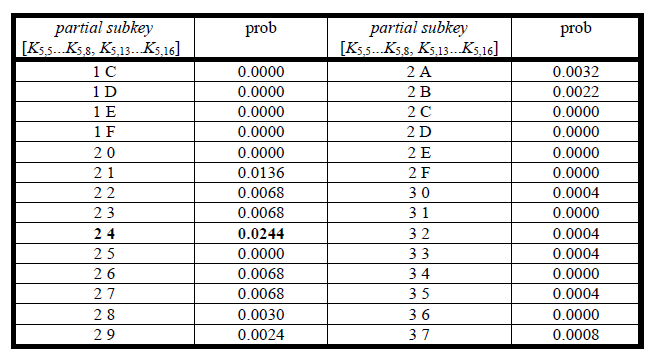
\includegraphics[width=1.0\linewidth]{experimental-results-for-differential-attack.PNG}
		\caption{Experimental Results for Differential Attack}
	\end{figure}
	
}
\section{Automatic Security Evaluation of Block Ciphers}
\frame { \frametitle{Introduction of MILP}
	\begin{itemize}
	\item Counting the number of active S-boxes is a common way to
	evaluate the security of symmetric key cryptographic schemes against differential
	attack. Based on Mixed Integer Linear Programming (MILP), we can the minimal number of active S-boxes. 
	~ \\
	~ \\
	\item MILP: Given $A \in \mathbb{R}^{m \times n}, b \in \mathbb{R}^{m}$ and $c_{1}, \cdots, c_{n} \in \mathbb{R}^{n}$, find an $x \in \mathbb{Z}^{k} \times \mathbb{R}^{n-k} \subseteq \mathbb{R}^{n} $ with $A x \leq b$, such that the linear function $c_{1} x_{1}+c_{2} x_{2}+\cdots+c_{n} x_{n}$ is minimized (or maximized) with respect to the linear constraint $A x \leq b$.
	\end{itemize}
}

\frame { \frametitle{Building the Model}
	\begin{itemize}
		\item For every input and output bit-level difference, a new 0-1 variable $x_{i}$ is introduced obeying the following rule of variable assignment.$$
		x_{i}=\left\{\begin{array}{l}{1, \text { for nonzero difference at this bit, }} \\ {0, \text { otherwise. }}\end{array}\right.$$
		~ \\
		~ \\
		\item For every S-box in the schematic diagram, including the encryption provess and the key schedule algorithm, we instroduce a new 0-1 variable $A_{j}$ such that $$
		A_{j}=\left\{\begin{array}{l}{1, \text { if the input word of the Sbox is nonzero, }} \\ {0, \text { otherwise. }}\end{array}\right.$$
		
		\item At this point, it is natural to choose the objective function $f$, which will be minimized, as $\sum A_{j}$ for the goal of determining a lower bound of the number of active S-boxes.$$Min \ f = \sum A_{j}$$
	\end{itemize}
}
\frame { \frametitle{Constrains Describing the S-box Operation}
	\begin{itemize}
		\item Suppose  $\left(x_{i_{0}}, \ldots, x_{i_{\omega-1}}\right)$ and $\left(y_{j_{0}}, \dots, y_{j_{\nu-1}}\right)$ are the input and output bit-level differences of an $\omega \times \nu$ S-box marked by $A_{t}$. Firstly, to ensure that $A_{t}=1$ holds if and only if $\left(x_{i_{0}}, \ldots, x_{i_{\omega-1}}\right)$ are not all zero,we require that:$$
		\left\{\begin{array}{l}{A_{t}-x_{i_{k}} \geq 0, \quad k \in\{0, \ldots, \omega-1\}} \\ {x_{i_{0}}+x_{i_{1}}+\cdots+x_{i_{\omega-1}}-A_{t} \geq 0}\end{array}\right.$$
		~ \\ 
		~ \\
		\item For bijective S-boxes, nonzero input difference must result in nonzero output difference and vice versa: $$
		\left\{\begin{array}{l}{\omega y_{j 0}+\omega y_{j_{1}}+\cdots+\omega y_{j_{\omega-1}}-\left(x_{i_{0}}+x_{i_{1}}+\cdots+x_{i_{\omega-1}}\right) \geq 0} \\ {\nu x_{i_{0}}+\nu x_{i_{1}}+\cdots+\nu x_{i_{\omega-1}}-\left(y_{j_{0}}+y_{j_{1}}+\cdots+y_{j_{\nu-1}}\right) \geq 0}\end{array}\right.$$
	\end{itemize}
}
\frame { \frametitle{Constrains Describing the S-box Operation, cont}
	\begin{itemize} 
		\item The Hamming weight of the $(\omega+\nu)$-bit word $x_{i_{0}} \cdots x_{i_{\omega-1}}, y_{j_{0}} \cdots y_{j_{\nu-1}}$ is lower bounded by the branch number $\mathcal{B}_{\mathcal{S}}$ of the S-box for nonzero input difference $x_{i_{0}} \cdots x_{i_{\omega-1}}$, where $d_{\mathcal{S}}$ is a dummy variable:$$
		\left\{\begin{array}{l}{\sum_{k=0}^{\omega-1} x_{i_{k}}+\sum_{k=0}^{\nu-1} y_{j_{k}} \geq \mathcal{B}_{\mathcal{S}} d_{\mathcal{S}}} \\ {d_{\mathcal{S}} \geq x_{i_{k}}, \quad k \in\{0, \ldots, \omega-1\}} \\ {d_{\mathcal{S}} \geq y_{j_{k}}, \quad k \in\{0, \ldots, \omega-1\}}\end{array}\right.$$
		~ \\ 
		~ \\
		\item The branch number $\mathcal{B}_{\mathcal{S}}$ of an S-box $\mathcal{S}$ is defined as $$
		\mathcal{B}_{\mathcal{S}}=\min _{a \neq b}\left\{\operatorname{wt}\left((a \oplus b) \|(\mathcal{S}(a) \oplus \mathcal{S}(b)): a, b \in \mathbb{F}_{2}^{\omega}\right\}\right.$$ and $\mathrm{wt}(\cdot)$ is the standard Hamming wight of a $2\omega$-bit word.
	\end{itemize}
}
\frame { \frametitle{Constrains Imposed by XOR Operations}
	\begin{itemize} 
		\item Suppose $a \oplus b=c$, where $a, b, c \in \mathbb{F}_{2}^{\omega}$ are the input and output differences of the XOR operation, the following constraints will make sure that when $ a $, $ b $ and $ c $ are not all zero, then there are at least two of them are nonzero: $$
		\left\{\begin{array}{l}{a+b+c \geq 2 d_{\oplus}} \\ {d_{\oplus} \geq a} \\ {d_{\oplus} \geq b} \\ {d_{\oplus} \geq c}\end{array}\right.$$ where $d_{\oplus}$ is a dummy variable taking values from $\{0,1\}$. 
		~ \\ 
		~ \\
		\item If each one of $a,b$ and $c$ represents one bit, we should also add the inequalitie:
		$$a+b+c \leq 2$$
		
	\end{itemize}
}
\frame { \frametitle{Result for the single-key Present differential analysis}
	\begin{figure}[h]
		\centering  
		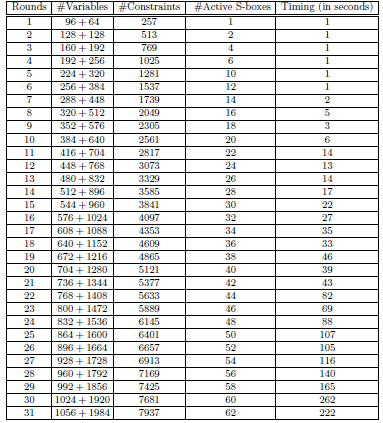
\includegraphics[width=0.5\linewidth]{present-differential-analysis.PNG}  
		\caption{Result for the single-key Present differential analysis}  
	\end{figure}
}

\section{Tighten the Feasible Region with Valid Cutting-off	Inequalities}
\frame { \frametitle{Valid Cutting-off Inequalities}
	\begin{figure}[h]
		\centering  
		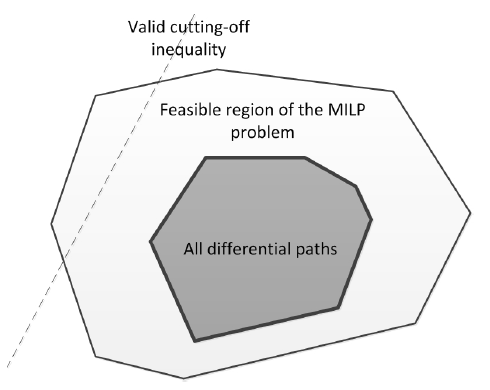
\includegraphics[width=0.6\linewidth]{valid-cutting-off-inequality.PNG}  
		\caption{The relationship between the set of all differential paths and the feasible region of the MILP problem, and the effect of cutting-off inequality }  
	\end{figure}
}
\frame { \frametitle{Methods for Generating Valid Cutting-off Inequalities}
	\begin{theorem}[1]
		The S-box of PRESENT-80 has the following properties: \\
		(i) $1001 \rightarrow ???0$: If the input difference of the S-box is $0x9=1001$, then the least significant bit of the output difference must be 0;\\
		(ii) $0001 \rightarrow ???1$: If the input difference of the S-box is $0x1=0001$ or $0x8=1000$, then the least significant bit of the output difference must be 1;\\
		(iii) $???1 \rightarrow 0001$ and $???1 \rightarrow 0100$: If the output difference of the S-box is $0x1=0001$ or $0x4=0100$, then the least significant bit of the input difference must be 1;\\
		(iiii) $???0 \rightarrow 0101$: If the output difference of the S-box is $0x5=0101$, then the
		least significant bit of the input difference must be 0.
	\end{theorem}
}
\frame { \frametitle{Methods for Generating Valid Cutting-off Inequalities, cont}
	\begin{theorem}[2]
		Let $0$-$1$ variables $\left(x_{0}, x_{1}, x_{2}, x_{3}\right)$ and $\left(y_{0}, y_{1}, y_{2}, y_{3}\right)$ represent the input and output differences of the S-box respectively, where $x_{3}$ and $y_{3}$ are the least significant bit. Then the logical conditions in Theorem 1 can be described by the following linear inequalities: $$	-x_{0}+x_{1}+x_{2}-x_{3}-y_{3}+2 \geq 0	$$
		
		$$\left\{\begin{array}{l}{x_{0}+x_{1}+x_{2}-x_{3}+y_{3} \geq 0} \\ {-x_{0}+x_{1}+x_{2}+x_{3}+y_{3} \geq 0}\end{array}\right.$$
		
		$$\left\{\begin{array}{l}{x_{3}+y_{0}+y_{1}+y_{2}-y_{3} \geq 0} \\ {x_{3}+y_{0}-y_{1}+y_{2}+y_{3} \geq 0}\end{array}\right.$$
		
		$$-x_{3}+y_{0}-y_{1}+y_{2}-y_{3}+2 \geq 0$$
	\end{theorem}
}

\frame { \frametitle{Convex Hull of All Possible Differentials for an S-box}
	\begin{itemize}
		\item The convex hull of a set $Q$ of discrete points in $\mathbb{R}^{n}$ is the smallest convex set that contains $Q$. A convex hull can be described as the common solutions of a set of finitely many linear euqations and inequalities as follows:	$$\left\{\begin{array}{l}{\lambda_{0,0} x_{0}+\cdots +\lambda_{0,n-1}x_{n-1}+\lambda_{0,n}\geq 0} \\ {\gamma_{0,0} x_{0}+\cdots +\gamma_{0,n-1}x_{n-1}+\gamma_{0,n} = 0}\end{array}\right.$$
		This is called the H-representation of a convex hull.
		~ \\ 
		~ \\
		\item Define the convex hull of a specfic $\omega \times \nu$ S-box to the set of all linear inequalities in the H-Representation of the convex hull $\nu_{S} \subseteq \mathbb{R}^{\omega+\nu}$ of all possible differential patterns of the S-box.
 	\end{itemize}
}

\frame { \frametitle{Convex Hull of All Possible Differentials for an S-box, cont}
	\begin{figure}[h]
		\centering  
		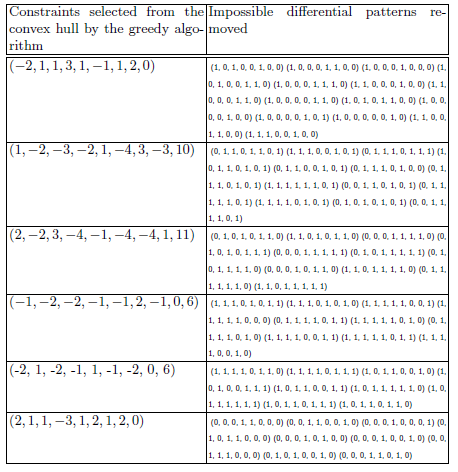
\includegraphics[width=0.6\linewidth]{convex-hull-remove-differential-pattern.PNG}  
		\caption{Impossible differential patterns removed by the constraints selected from the convex hull of the Present S-box}  
	\end{figure}
}
\frame { \frametitle{Convex Hull of All Possible Differentials for an S-box, cont}
	\begin{figure}[h]
		\centering  
		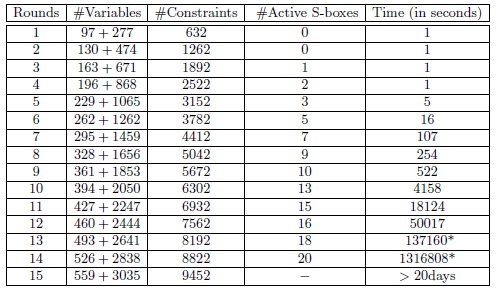
\includegraphics[width=0.7\linewidth]{milp-present-with-cdp-constraints.PNG}  
		\caption{MILP related-key models for Present with CDP constraints added}  
	\end{figure}
}
\section{NBC}
\frame { \frametitle{NBC}
	\begin{figure}[h]
		\centering  
		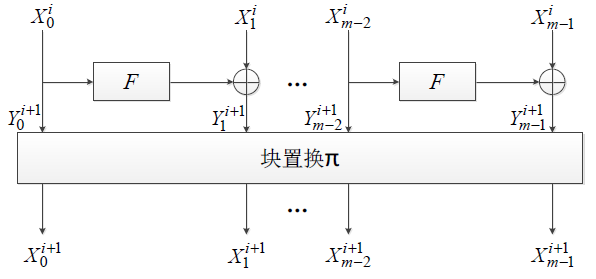
\includegraphics[width=0.6\linewidth]{NBC-Function.PNG}  
		\caption{NBC Round Function }  
	\end{figure}
	\begin{figure}[h]
	\centering  
	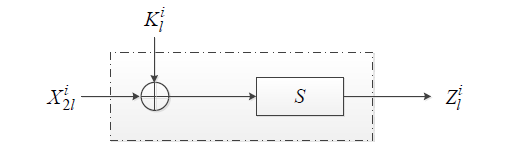
\includegraphics[width=0.6\linewidth]{NBC-F-Function.PNG}  
	\caption{F Function }  
	\end{figure}
}
\frame { \frametitle{NBC-128}
	\begin{figure}[h]
		\centering  
		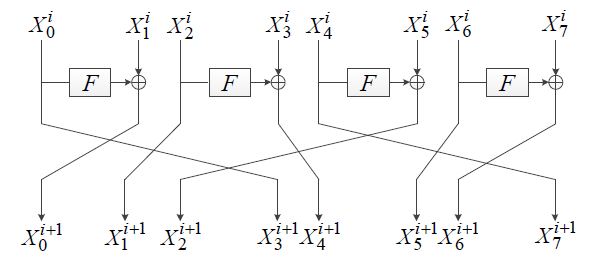
\includegraphics[width=0.6\linewidth]{NBC-128-F-Function.PNG}  
		\caption{NBC-128 Round Function }  
	\end{figure}
	\begin{figure}[h]
		\centering  
		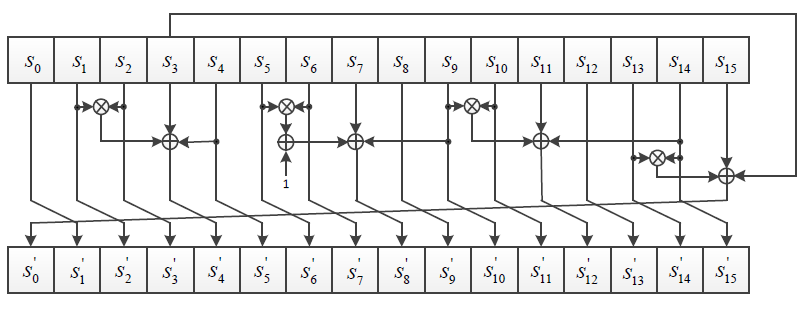
\includegraphics[width=0.6\linewidth]{NBC-S-box.PNG}  
		\caption{NBC-128 S-box }  
	\end{figure}
}
\end{document}

